	\chapter{Kravspecifikation}
	
		\section{Systembeskrivelse}
				Systemet består af en database med brugeradgang via web- eller Android applikation.
				Databasen indeholder brugere, sager og data om lysreguleringerne.
				En sag indeholder en fejlkode, kommentarfelt, mulighed for upload af billede og status.
				Der er fire tilstande af status som en sag kan have: Oprettet, Påbegyndt, Afventer og Afsluttet. På figur \ref{fig:OversigtSystembeskrivelsen} beskrives sammenhængen mellem enhederne i systemet.
				
				\begin{figure}[H]
					\centering
					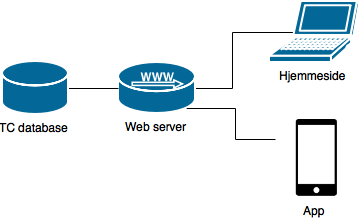
\includegraphics[width=0.6\linewidth]{Kravspecifikation/Oversigtoversystem}
					\caption{Oversigt over systemet}
					\label{fig:OversigtSystembeskrivelsen}
				\end{figure}
				
				Systemet skal kunne oprette sager, når Randers Kommune modtager en fejlmeddelelse.
				Disse skal kunne tilgås af Strøm Hansen og Randers Kommune gennem den ønskede bruger adgang via PC eller smartphone.
				Systemet skal kunne notificere Strøm Hansen og Randers Kommune, når der foretages reparationer på en given sag. Notifikationen vil være igennem enten Android applikationen, e-mail eller SMS.
				Montørerne bliver tildelt et personligt log ind, som skal bruges når de foretager en reparation på en given sag.
				Montøren har mulighed for at ændre status på en oprettet sag. Derudover har montøren mulighed for at uploade relevante billeder og skrive kommentarer til reparationen.
				Systemet har en log, som indeholder en liste over alle sager, hvori det vil være muligt at søge og sortere i.
				
					
				\section{Afgrænsning}
				Projektet har en naturlig begrænsning i form af den korte tid fra idé til produkt, som er gældende for semesterprojekter. 
				
				Web applikationen vil blive udviklet med ASP.NET MVC. 
				Smartphone applikationen vil blive udviklet til Android. Til Android anvendes Xamarin, det muliggør at skrive i C\#.
				Både web- og android applikationen vil have et grafisk brugergrænseflade (GUI). Web applikationen vil kunne skalere opløsningen alt efter hvilken enhed applikationen tilgås fra.\\

	
	\section{User stories} 
	Følgende er en beskrivelse kort af user stories til Traffic Control. For fuldt beskrevet user stories med Gherkin, se dokumentationen afsnit \vref{Dok-sec:UserStories}.
	Aktør kontekst diagram findes i dokumentationen afsnit \vref{Dok-sec:aktor}.

	\subsection*{Log-in}
	Som bruger\\
	Ønsker jeg at kunne logge ind på applikationen\\
	For at kunne benytte applikationen
	
	\subsection*{Opret bruger}
	Som ejer\\
	Ønsker jeg at kunne oprette bruger på applikationen\\
	For at kunne give montører samt kunder adgang til systemet
	
	\subsection*{Ændring af brugeroplysninger}
	Som bruger\\
	Ønsker jeg at kunne ændre brugeroplysninger\\
	For at have aktuelle oplysninger på applikationen
	
	\subsection*{Opret en sag}
	Som ejer eller montør\\
	Ønsker jeg at kunne oprette en sag\\
	For kunne lave en fejlmelding på et given lyskryds

	\subsection*{Tag en sag}
	Som montør\\
	Ønsker jeg at kunne tage en sag\\
	For at kunne lave en reparation på et fejlmeldt lyskryds
	
	\subsection*{Ændring af en sags driftstatus}
	Som montør\\
	Ønsker jeg at kunne ændre en sags driftstatus\\
	For at kunne holde Strøm Hansen og Randers kommune opdateret på reparatoioner af lyskryds
	
	\subsection*{Skrive kommentar til en sag}
	Som bruger\\
	Ønsker jeg at kunne skrive kommentar til en given sag\\
	For at kunne skrive kommentar på eventuelle mangler, feedback og til korrespondance mellem de forskellige brugere.

	\subsection*{Sortere sager}
	Som bruger\\
	Ønsker jeg at kunne sortere sager\\
	For at give et hurtigt overblik hvis en specifik sag ønskes fundet

	\subsection*{Få overblik ved hjælp af et map}
	Som bruger\\
	Ønsker jeg at kunne danne mig et hurtigt overblik ved hjælp af en map funktion\\
	For at kunne se et overbliks billede af alle lyskryds i Randers kommune  og deres nuværende status
	
	\subsection*{Modtage notifikationer om ændrede driftstatus}
	Som kunde og ejer\\
	Ønsker jeg at modtage notifikationer når en driftstatus ændre sig på et lyskryds ændre sig\\
	For at få opdateringer hvis et lyskryds ændre driftstatus
	
	\subsection*{Information omkring lyskryds}
	Som bruger\\
	Ønsker jeg at kunne skrive generelle informationer eller kommentar til et specifikt lyskryds\\
	For at kunne videre give kommentar som er specifike for det enkelte lyskryds

	\section{Ikke funktionelle krav}
	\begin{itemize}[-]
		\itemsep 0.3em 
		\item Skal kunne tilgås gennem en Web applikation og Android applikation
		\item Der skal anvendes Microsoft teknologier og software
		\item Alle brugere skal kunne anvende systemet på samme tid. Maks antal enheder er 100 på samme tid
		\item Systemet skal have svartider under 500ms ved 99\% af requests på en dansk kablet internetforbindelse
		\item Systemet skal have en oppetid på 99,7\%, målt over 3 måneder
		\item Database og web-server skal være køre på hver deres server
		\item Domænet trafficcontrol.dk skal anvendes
	\end{itemize}
	